% Copyright 2004 by Till Tantau <tantau@users.sourceforge.net>.
%
% In principle, this file can be redistributed and/or modified under
% the terms of the GNU Public License, version 2.
%
% However, this file is supposed to be a template to be modified
% for your own needs. For this reason, if you use this file as a
% template and not specifically distribute it as part of a another
% package/program, I grant the extra permission to freely copy and
% modify this file as you see fit and even to delete this copyright
% notice. 

\documentclass{beamer}

% There are many different themes available for Beamer. A comprehensive
% list with examples is given here:
% http://deic.uab.es/~iblanes/beamer_gallery/index_by_theme.html
% You can uncomment the themes below if you would like to use a different
% one:
%\usetheme{AnnArbor}
%\usetheme{Antibes}
%\usetheme{Bergen}
%\usetheme{Berkeley}
%\usetheme{Berlin}
%\usetheme{Boadilla}
%\usetheme{boxes}
%\usetheme{CambridgeUS}
%\usetheme{Copenhagen}
%\usetheme{Darmstadt}
%\usetheme{default}
%\usetheme{Frankfurt}
%\usetheme{Goettingen}
%\usetheme{Hannover}
%\usetheme{Ilmenau}
%\usetheme{JuanLesPins}
%\usetheme{Luebeck}
%\usetheme{Madrid}
%\usetheme{Malmoe}
%\usetheme{Marburg}
%\usetheme{Montpellier}
%\usetheme{PaloAlto}
%\usetheme{Pittsburgh}
%\usetheme{Rochester}
\usetheme{Singapore}
%\usetheme{Szeged}
%\usetheme{Warsaw}

\usefonttheme[onlymath]{serif}
\usepackage{stmaryrd}


\title{Multiresolution Kernel Approximation for\\ Gaussian Process Regression}



\author{Yi Ding\inst{1} \and Risi Kondor\inst{1}\inst{2} \and Jonathan Eskreis-Winkler\inst{2}}
% - Give the names in the same order as the appear in the paper.
% - Use the \inst{?} command only if the authors have different
%   affiliation.

\institute[Universities of Somewhere and Elsewhere] % (optional, but mostly needed)
{
  \inst{1}%
  Department of Computer Science\\
  \inst{2}%
  Department of Statistics\\
  The University of Chicago}
% - Use the \inst command only if there are several affiliations.
% - Keep it simple, no one is interested in your street address.

\date{presenter:\\
Niklas Schmitz\\
Seminar Hot Topics in Machine Learning\\
summer term 2019, TU Berlin}
% - Either use conference name or its abbreviation.
% - Not really informative to the audience, more for people (including
%   yourself) who are reading the slides online


\subject{Theoretical Computer Science}
% This is only inserted into the PDF information catalog. Can be left
% out. 

% If you have a file called "university-logo-filename.xxx", where xxx
% is a graphic format that can be processed by latex or pdflatex,
% resp., then you can add a logo as follows:

% \pgfdeclareimage[height=0.5cm]{university-logo}{university-logo-filename}
% \logo{\pgfuseimage{university-logo}}

% Delete this, if you do not want the table of contents to pop up at
% the beginning of each subsection:
%\AtBeginSubsection[]
%{
%  \begin{frame}<beamer>{Outline}
%    \tableofcontents[currentsection,currentsubsection]
%  \end{frame}
%}

% Let's get started
\begin{document}

\begin{frame}
  \titlepage
\end{frame}

\begin{frame}{Outline}
  \tableofcontents
  % You might wish to add the option [pausesections]
\end{frame}

% Section and subsections will appear in the presentation overview
% and table of contents.

%%%%%%%%%%%%%%%%%%%%%%%%%%%%%%%%%%%%%%%%%%%%%%%%%%%%%%%%%%%%%%%%%%%%%%%%%%%%%%%%%%%%%%%%%%%%%%%%%%%%%
\section{Motivation}
%%%%%%%%%%%%%%%%%%%%%%%%%%%%%%%%%%%%%%%%%%%%%%%%%%%%%%%%%%%%%%%%%%%%%%%%%%%%%%%%%%%%%%%%%%%%%%%%%%%%%

\subsection{Gaussian Process Regression}

\begin{frame}{Gaussian Process}
\begin{block}{Definition (Gaussian Process)}
    A Gaussian process is a collection of random variables, any
    finite number of which have a joint Gaussian distribution
\end{block}
    
\end{frame}

\begin{frame}{Recap: Gaussian Process}
  Recall that a Gaussian Process (GP) on a space $\mathcal{X}$ is a prior over functions $f: \mathcal{X}\to \mathbb{R}$ fully specified by\pause
  \begin{itemize}
      \item<2-> mean function: $\mu(x) = \mathbb{E}[f(x)]$
      \item<3-> covariance function: $k(x,x') = Cov(f(x), f(x'))$
  \end{itemize}
\end{frame}

\begin{frame}{Recap: Gaussian Process Regression}
    Given:
    \begin{itemize}
        \item training data $\{(x_1,y_1),\hdots ,(x_n,y_n)\}$
        \item model $y_i=f(x_i)+\epsilon$ with noise $\epsilon \sim \mathcal{N}(0,\sigma^2)$
    \end{itemize}
    The posterior is also a GP with\pause
    \begin{itemize}
        \item $\mu'(x) = \mu(x) + \mathbf{k_x}^\top(K+\sigma^2I)^{-1}y$
        \item $k'(x,x') = \mathbf{k_{x'}}^\top(K+\sigma^2I)^{-1}\mathbf{k_x}$
    \end{itemize}
    where $\mathbf{k_x}=(k(x,x_1),\hdots,k(x,x_n)^\top$, $y=(y_1,\hdots,y_n)^\top$
\end{frame}


\begin{frame}{Recap: Gaussian Process Regression}
\begin{figure}
    \centering
     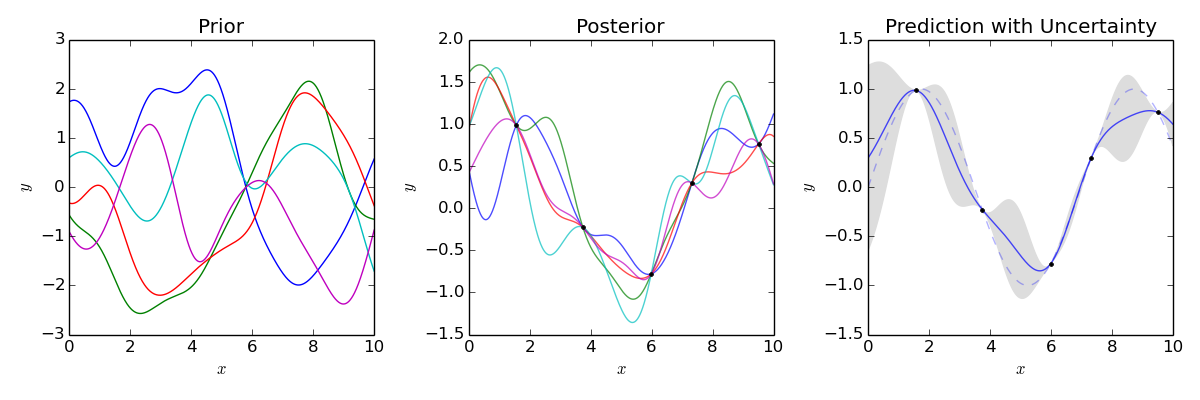
\includegraphics[scale=0.35]{figs/Gaussian_Process_Regression.png}
\end{figure}
With $\mu(x)=0$ the posterior mean estimate is
\begin{align*}
    \hat{f}(x)=\mathbf{k_x}^\top(K+\sigma^2I)^{-1}y
\end{align*}
\\\\
\tiny\textcolor{gray}{image source: \url{https://commons.wikimedia.org/wiki/File:Gaussian_Process_Regression.png}}

\end{frame}
%%%%%%%%%%%%%%%%%%%%%%%%%%%%%%%%%%%%%%%%%%%%%%%%%%%%%%%%%%%%%%%%%%%%%%%%%%%%%%%%%%%%%%%%%%%%%%%%%%%%%
\section{Low Rank Approximations}
%%%%%%%%%%%%%%%%%%%%%%%%%%%%%%%%%%%%%%%%%%%%%%%%%%%%%%%%%%%%%%%%%%%%%%%%%%%%%%%%%%%%%%%%%%%%%%%%%%%%%

%--------------------------------------------------
\subsection{Global Low Rank Methods: Nystr\"om}
%--------------------------------------------------

\begin{frame}{Nystr\"om Approximation}
    \begin{itemize}
        \item Intuition: $k(x,x')$ encodes similarity between points
        \item For a smooth, slowly varying $k$: use data subset as pseudo-inputs 
            $\{x_{i_1},...,x_{i_m}\}$ to approximate $k(x,x')$
    \end{itemize}
\end{frame}

\begin{frame}{Nystr\"om Approximation}
For a smooth, slowly varying $k$: use subset of training data as pseudo-inputs 
            $\{x_{i_1},...,x_{i_m}\}$ to approximate $k(x,x')$
    \begin{align*}
        k(x,x') \approx \sum_{s=1}^{m}\sum_{j=1}^{m} k(x,x_{i_s})c_{i_s,i_j}k(x_{i_j},x')
    \end{align*}
    or in matrix form $K \approx K_{*,I}CK_{*,I}^\top$. When $C=K_{I,I}^+$ one obtains the canonical Nystr\"om approximation:
    \begin{align*}
        K \approx K_{*,I}K_{I,I}^+K_{*,I}^\top
    \end{align*}
\end{frame}

% efficiency

% choosing landmark set I is another problem

% fundamental limitation: inherently low rank. (no reason to believe that K is well approximated)

\begin{frame}{Nystr\"om Approximation}
    \begin{align*}
        K \approx K_{*,I}K_{I,I}^+K_{*,I}^\top
    \end{align*}
    \begin{itemize}
        \item simple, reliable performance bounds
        \item inherently low rank
    \end{itemize}
    \pause
    Finding a good set $I$ of landmark points is critical
    \pause
    \begin{block}{Remark}
     There is no reason to believe that K is close to low rank in general!
    \end{block}
   
\end{frame}

% PCA-like vs kNN-like

%---------------------------------------------------
\subsection{Local and Hierarchical Low Rank Methods}
%---------------------------------------------------

\begin{frame}{Local approximation}
    \begin{enumerate}
        \item cluster rows/columns by some fast method
        \item compute diagonal blocks $\llbracket K\rrbracket_{i,i}\approx U_i\Sigma_iU_i^T$
        \begin{itemize}
            \item low rank, but relatively high accuracy
        \end{itemize}
        \item compute off diagonal blocks $\llbracket K\rrbracket_{i,j}$ from bases $\{U_i\}$
    \end{enumerate}
\end{frame}
% inherently parallelizable

% natural extension: apply divide&conquer approach on multiple scales


\begin{frame}{Local and Hierarchical low rank methods}
    
    \begin{figure}
        \centering
        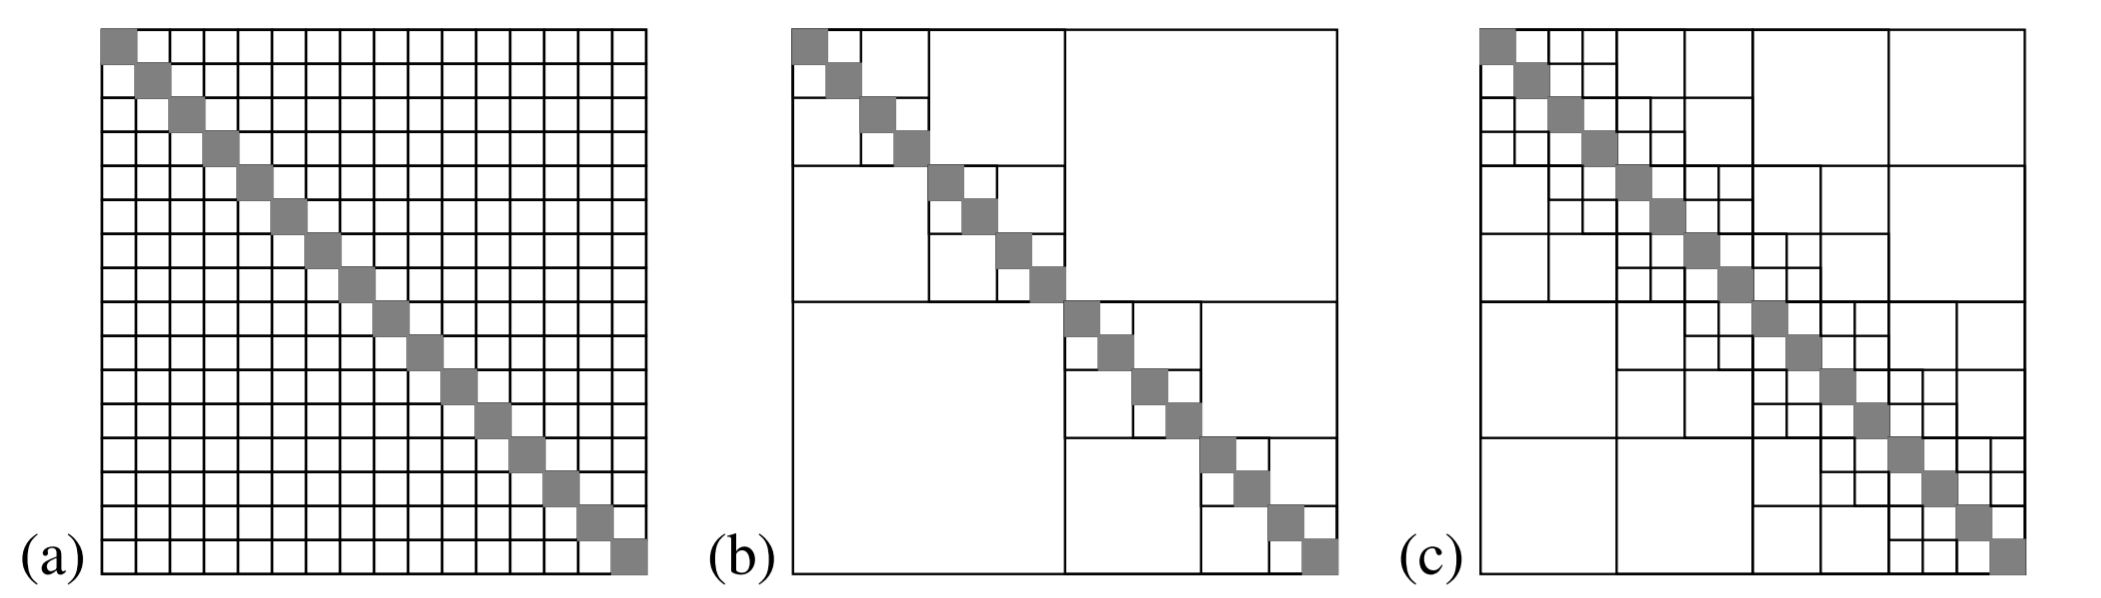
\includegraphics[scale=0.15]{figs/matrixsketch.png}
        \label{fig:my_label}
    \end{figure}
    (a) In a simple blocked low rank approximation the diagonal blocks
    are dense (gray)\\
    (b) In an HODLR matrix the low rank off-diagonal blocks form a hierarchical structure leading to a much more compact representation.\\
    (c) H2 matrices are a refinement of this idea
    
\end{frame}

%%%%%%%%%%%%%%%%%%%%%%%%%%%%%%%%%%%%%%%%%%%%%%%%%%%%%%%%%%%%%%%%%%%%%%%%%%%%%%%%%%%%%%%%%%%%%%%%%%%%%
\section{Multiresolution Kernel Approximation}
%%%%%%%%%%%%%%%%%%%%%%%%%%%%%%%%%%%%%%%%%%%%%%%%%%%%%%%%%%%%%%%%%%%%%%%%%%%%%%%%%%%%%%%%%%%%%%%%%%%%%

\begin{frame}{Multiresolution Kernel Approximation (MKA)}
    \begin{itemize}
        \item data adapted, multiscale approach
        \item distant clusters interact in a low rank fashion
        \item more flexible than existing hierarchical approaches: 
    \end{itemize}
\end{frame}

%---------------------------------------------------
\subsection{c-core-diagonal compression}
%---------------------------------------------------

\begin{frame}{Multiresolution Kernel Approximation (MKA)}
    \begin{block}{Definition 1}
     A matrix $H$ is \textbf{c-core-diagonal} if $H_{i,j}=0$ unless either $i,j\leq c$ or $i=j$
    \end{block}
    \begin{block}{Definition 2}
     A \textbf{c-core-diagonal compression} of a symmetric matrix $A\in\mathbb{R}^{m\times m}$ is an approximation of the form
    \begin{figure}
        \centering
        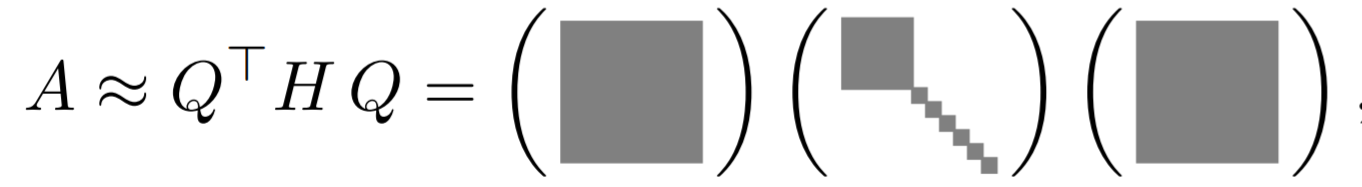
\includegraphics[width=0.8\linewidth]{figs/ccore.png}
    \end{figure}
    where Q is orthogonal and H is c-core-diagonal.
    \end{block}
\end{frame}

\begin{frame}{Multiresolution Kernel Approximation (MKA)}
\begin{itemize}
    \item Hierarchical approaches apply low rank approximations to many blocks of $K$ in parallel, at different scales
    \item  MKA works similarly, but applies core-diagonal compressions
    \pause
    \item $K$ is taken through a series of transformations called stages
\end{itemize}
\begin{align*}
    \Tilde{K}=K_0\mapsto K_1\mapsto\hdots\mapsto K_s
\end{align*}
\end{frame}

%---------------------------------------------------
\subsection{the MKA algorithm}
%---------------------------------------------------

\begin{frame}{Multiresolution Kernel Approximation (MKA)}
At each stage $s$:
    \begin{enumerate}
        \item cluster rows/columns of $K_{s-1}$ to form blocked matrix $\overline{K_{s-1}}=C_sK_{s-1}C_s^\top$ where $\llbracket \overline{K}_{s-1}\rrbracket_{i,j}=[K_{s-1}]_{C_i^s, C_j^s}$
        \item compress diagonal blocks of $\overline{K_{s-1}}$ to c-core-diagonal form $\llbracket K\rrbracket_{i,i}\approx Q_i\llbracket K_{s-1}\rrbracket_{i,i}Q_i^\top$ (e.g. through MMF\cite{kondor2014multiresolution})
    \end{enumerate}
\end{frame}

\begin{frame}{Multiresolution Kernel Approximation (MKA)}
At each stage $s$:
    \begin{enumerate} \setcounter{enumi}{2}
        \item assemble local rotations $Q_i^s$ into large orthogonal matrix $\overline{Q_s}=\bigoplus_i Q_i^s$ and applied give $\overline{H_s}=\overline{Q_s}\,\overline{K_{s-1}}\,\overline{Q_s}^\top$\pause
        \item permute $\overline{H_1}$ by mapping the core part of each block to one of the first $c_s:=c_1^s_\hdots c_{p_s}^s$, giving $H_s^{pre}=P_s\overline{H_s}P_s^\top$\pause
        \item Truncate $H_s^{pre}$ into core-diagonal form $H_s=K_s\oplus D_s$, where $K_s\in\mathbb{R}^{c_s\times c_s}$ is dense while $D_s$ is diagonal. Together this gives a core-diagonal compression of the previous stage
        \begin{align*}
          K_{s-1} = \underbrace{C_s^\top \overline{Q_s}^\top P_s^\top}_{Q_s^\top} (K_s \oplus D_s)\underbrace{P_s \overline{Q_s} C_s}_{Q_s^\top}
        \end{align*}
    \end{enumerate}
\end{frame}

\begin{frame}{Multiresolution Kernel Approximation (MKA)}
    The kernel approximation $\Tilde{K}$ takes a telescoping form
\begin{align*}
\Tilde{K} \approx Q_1^\top(Q_2^\top(\hdots Q_s^\top(K_s\oplus D_s)Q_s\hdots\oplus D_2)Q_2\oplus D_1)Q_1
\end{align*}
\begin{itemize}
    \item this makes computing its inverse efficient with $\mathcal{O}(n+d_{core}^3)$ operations
\end{itemize}
\end{frame}

\begin{frame}{MKA-GPs}
\begin{align*}
    \hat{f}(x)=\mathbf{k_x}^\top(K+\sigma^2I)^{-1}y
\end{align*}
\begin{itemize}
    \item now can compute $\check K=\mathit{MKA}(K+\sigma^2I)$ roughly in $\mathcal{O}(sn^2)$
    \item invert $\check K$ in $\mathcal{O}(n+d_{core}^3)$
    \item multiply $y$ by $\check{K}^{-1}$ in $\mathcal{O}(sn+d_{core}^2)$
\end{itemize}
\pause
\begin{block}{Remark}
using the Schur complement in the joint train/test kernel matrix it is possible in $\mathcal{O}((n+p)^2)$
% which is nice for less systematic bias of the approximation
\end{block}
\end{frame}


%%%%%%%%%%%%%%%%%%%%%%%%%%%%%%%%%%%%%%%%%%%%%%%%%%%%%%%%%%%%%%%%%%%%%%%%%%%%%%%%%%%%%%%%%%%%%%%%%%%%%
\section{Experimental Results}
%%%%%%%%%%%%%%%%%%%%%%%%%%%%%%%%%%%%%%%%%%%%%%%%%%%%%%%%%%%%%%%%%%%%%%%%%%%%%%%%%%%%%%%%%%%%%%%%%%%%%

\begin{frame}{Experimental Results}
    \begin{figure}
        \centering
        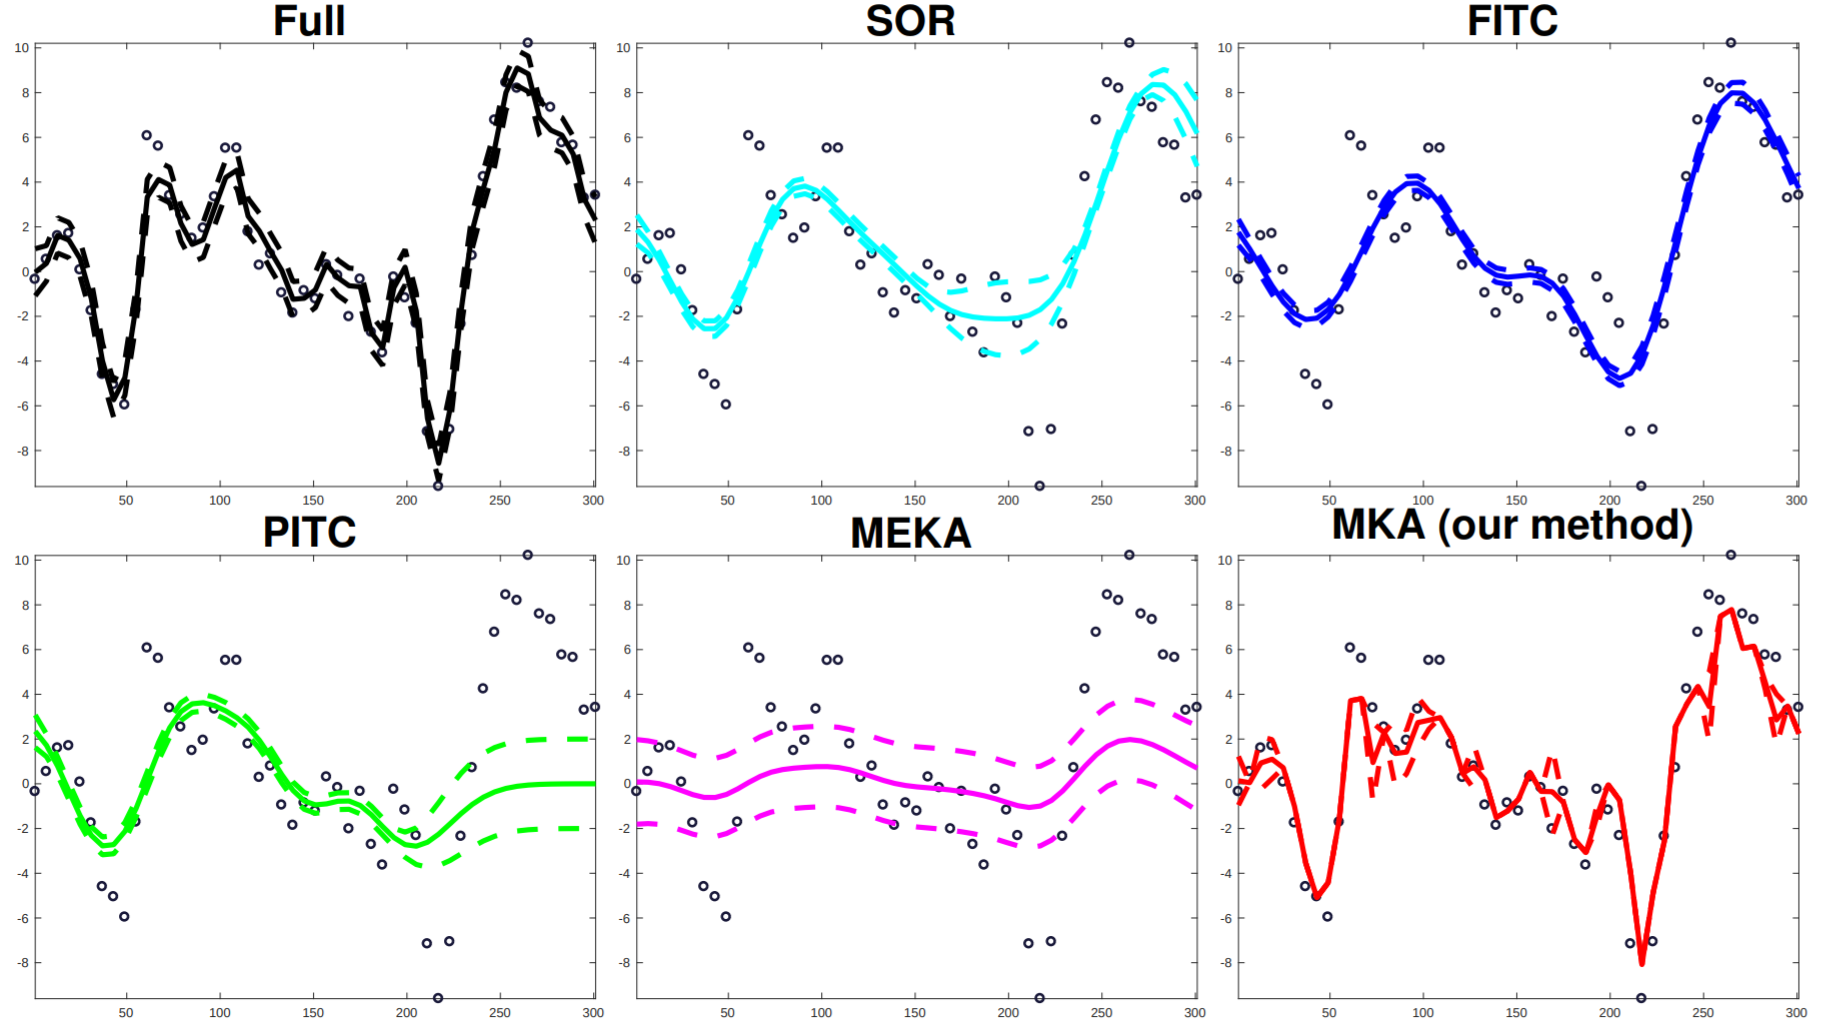
\includegraphics[width=0.8\linewidth]{figs/toyexample.png}
        \caption{Snelson's 1D example}
    \end{figure}
    MKA clearly outperforms existing approximations in being faithful to the full inference
\end{frame}

\begin{frame}{Experimental Results}
    \begin{figure}
        \centering
        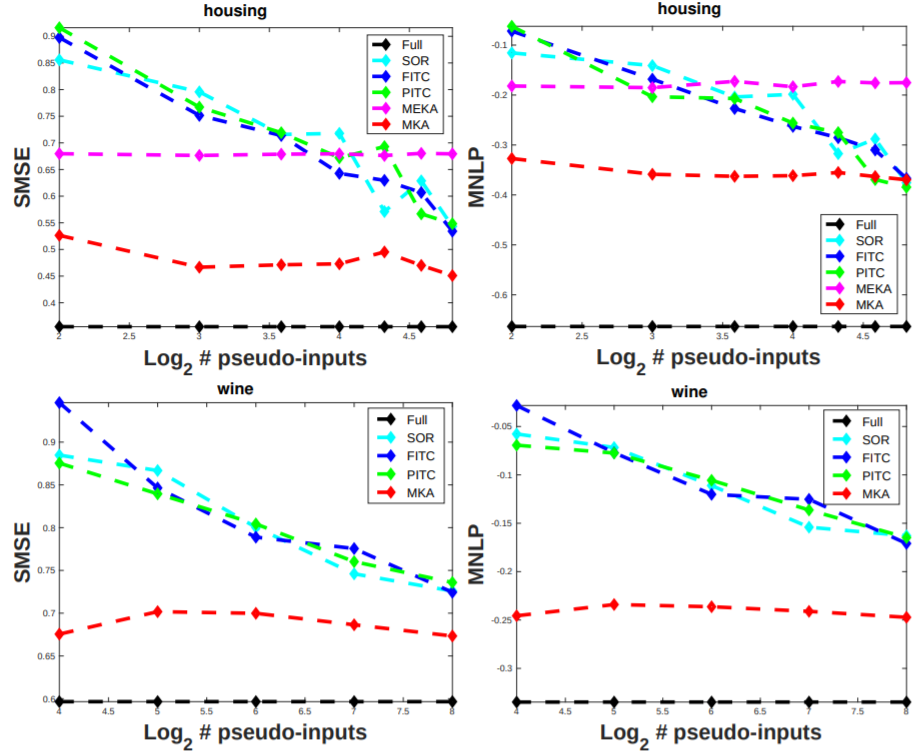
\includegraphics[width=0.6\linewidth]{figs/realdata.png}
        \caption{SMSE and MNLP as a function of the number of pseudo-inputs/dcore on two datasets}
    \end{figure}
\end{frame}


% Placing a * after \section means it will not show in the
% outline or table of contents.
%%%%%%%%%%%%%%%%%%%%%%%%%%%%%%%%%%%%%%%%%%%%%%%%%%%%%%%%%%%%%%%%%%%%%%%%%%%%%%%%%%%%%%%%%%%%%%%%%%%%%
\section*{Conclusions}
%%%%%%%%%%%%%%%%%%%%%%%%%%%%%%%%%%%%%%%%%%%%%%%%%%%%%%%%%%%%%%%%%%%%%%%%%%%%%%%%%%%%%%%%%%%%%%%%%%%%%

\begin{frame}{Conclusions}
\begin{itemize}
    \item MKA is a broad bandwith kernel approximation
    \item its factorization allows fast direct calculations of inverses and determinants, which are almost always the computational bottlenecks of Gaussian Processes
    \item in the presented experiments it outperforms low rank approximations, while only having a small computational overhead
\end{itemize}
\end{frame}


%%%%%%%%%%%%%%%%%%%%%%%%%%%%%%%%%%%%%%%%%%%%%%%%%%%%%%%%%%%%%%%%%%%%%%%%%%%%%%%%%%%%%%%%%%%%%%%%%%%%%
%%%%%%%%%%%%%%%%%%%%%%%%%%%%%%%%%%%%%%%%%%%%%%%%%%%%%%%%%%%%%%%%%%%%%%%%%%%%%%%%%%%%%%%%%%%%%%%%%%%%%

% All of the following is optional and typically not needed. 
\appendix
\section<presentation>*{\appendixname}
\subsection<presentation>*{For Further Reading}

\begin{frame}[allowframebreaks]
    \frametitle{References}
    \nocite{*}
    \bibliographystyle{unsrt}
    \bibliography{references}
\end{frame}

\end{document}


